\documentclass{Configuration_Files/PoliMi3i_thesis}

%------------------------------------------------------------------------------
%	REQUIRED PACKAGES AND  CONFIGURATIONS
%------------------------------------------------------------------------------

% CONFIGURATIONS
\usepackage{parskip} % For paragraph layout
\usepackage{setspace} % For using single or double spacing
\usepackage{emptypage} % To insert empty pages
\usepackage{multicol} % To write in multiple columns (executive summary)
 
\setlength\columnsep{15pt} % Column separation in executive summary
\setlength\parindent{0pt} % Indentation
\raggedbottom  

% PACKAGES FOR TITLES
\usepackage{titlesec}
% \titlespacing{\section}{left spacing}{before spacing}{after spacing}
\titlespacing{\section}{0pt}{3.3ex}{2ex}
\titlespacing{\subsection}{0pt}{3.3ex}{1.65ex}
\titlespacing{\subsubsection}{0pt}{3.3ex}{1ex}
\usepackage{color}

% PACKAGES FOR LANGUAGE AND FONT
\usepackage[english]{babel} % The document is in English  
\usepackage[utf8]{inputenc} % UTF8 encoding
\usepackage[T1]{fontenc} % Font encoding
\usepackage[11pt]{moresize} % Big fonts
\usepackage{beramono} % texttt font.


% PACKAGES FOR IMAGES
\usepackage{graphicx}
\usepackage{transparent} % Enables transparent images
\usepackage{eso-pic} % For the background picture on the title page
\usepackage{subfig} % Numbered and caption subfigures using \subfloat.
\usepackage{tikz} % A package for high-quality hand-made figures.
\usetikzlibrary{}
\graphicspath{{./Images/}} % Directory of the images
\usepackage{caption} % Coloured captions
\usepackage[dvipsnames]{xcolor} % clour using name for json like doc
\usepackage{amsthm,thmtools,xcolor} % Coloured "Theorem"
\usepackage{float}

% STANDARD MATH PACKAGES
\usepackage{amsmath}
\usepackage{amsthm}
\usepackage{amssymb}
\usepackage{amsfonts}
\usepackage{bm}
\usepackage[overload]{empheq} % For braced-style systems of equations.
\usepackage{fix-cm} % To override original LaTeX restrictions on sizes

% PACKAGES FOR TABLES
\usepackage{tabularx}
\usepackage{longtable} % Tables that can span several pages
\usepackage{colortbl}


% PACKAGES FOR ALGORITHMS (PSEUDO-CODE)
\usepackage{algorithm}
\usepackage{algorithmic}

% PACKAGES FOR REFERENCES & BIBLIOGRAPHY
\usepackage[colorlinks=true,linkcolor=black,anchorcolor=black,citecolor=black,filecolor=black,menucolor=black,runcolor=black,urlcolor=black]{hyperref} % Adds clickable links at references
\usepackage{cleveref}
\usepackage[square, numbers, sort&compress]{natbib} % Square brackets, citing references with numbers, citations sorted by appearance in the text and compressed
\bibliographystyle{abbrvnat} % You may use a different style adapted to your field

% OTHER PACKAGES
\usepackage{pdfpages} % To include a pdf file
\usepackage{afterpage}
\usepackage{lipsum} % DUMMY PACKAGE
\usepackage{fancyhdr} % For the headers
\fancyhf{}
\usepackage{array}
\usepackage{colortbl}
\usetikzlibrary{positioning, arrows.meta}

\usepackage{ulem}

% Define JSON key styles
\newcommand{\jsonkey}[1]{\textcolor{RoyalBlue}{\texttt{"#1"}}}
% Define JSON value styles
\newcommand{\jsonstring}[1]{\textcolor{ForestGreen}{\texttt{"#1"}}}
\newcommand{\jsonnumber}[1]{\textcolor{BrickRed}{\texttt{#1}}}
\newcommand{\jsonboolean}[1]{\textcolor{OrangeRed}{\texttt{#1}}}
\newcommand{\jsonnull}[1]{\textcolor{Gray}{\texttt{#1}}}

\usepackage{listings}
% Global settings shared between all code listings
\lstset{
    basicstyle=\ttfamily\small,        % Font style and size for all code
    numbers=left,                      % Line numbers on the left
    numberstyle=\tiny\color{gray},     % Style for line numbers
    breaklines=true,                   % Automatic line breaking
    showstringspaces=false,            % Do not show spaces in strings
    frame=lines                        % Draw a frame around the code
}

% Python-specific settings
\lstdefinelanguage{Python}{
    morekeywords={import, def, return, if, else, for, while, break, continue, class, lambda, pass},
    sensitive=true,
    morecomment=[l]{\#},
    morestring=[b]',
    morestring=[b]",
    keywordstyle=\color{blue},         % Python keywords in blue
    stringstyle=\color{green!70!black},% Strings in green
    commentstyle=\color{gray}          % Comments in gray
}

% MongoDB-specific settings
\lstdefinelanguage{MongoDB}{
    morekeywords={ db, find, insert, update, delete, aggregate, 
        \$match, \$group, \$project, \$sort, \$limit, \$skip, \$unwind, \$lookup, \$facet, \$bucket, \$bucketAuto, \$replaceRoot, \$merge, \$addFields, \$count, \$sortByCount, \$out,
        \$eq, \$ne, \$gt, \$gte, \$lt, \$lte, \$in, \$nin, \$and, \$or, \$not, \$nor, \$exists, \$type, \$regex, \$expr, \$mod, \$all, \$size, \$elemMatch,
        \$set, \$unset, \$inc, \$mul, \$rename, \$push, \$pull, \$addToSet, \$pop, \$pullAll, \$currentDate, \$min, \$max,
        \$elemMatch, \$size, \$all, \$arrayElemAt, \$concatArrays, \$filter, \$slice, \$map, \$reduce,
        \$add, \$subtract, \$multiply, \$divide, \$mod, \$sum,
        \$concat, \$substr, \$toLower, \$toUpper, \$strLenCP, \$trim, \$ltrim, \$rtrim, \$regexFind, \$regexMatch,
        \$dateFromString, \$dateToString, \$dayOfMonth, \$dayOfWeek, \$dayOfYear, \$hour, \$isoDayOfWeek, \$isoWeek, \$isoWeekYear, \$minute, \$month, \$second, \$millisecond, \$week, \$year,
        \$cond, \$ifNull, \$switch,
        \$literal, \$mergeObjects, \$range, \$zip, \$type},
    sensitive=true,
    morecomment=[l]{//},
    morestring=[b]",
    keywordstyle=\bfseries\color{blue}, % MongoDB keywords in bold blue
    stringstyle=\color{green!70!black},            % Strings in green
    commentstyle=\color{gray},          % Comments in gray
    backgroundcolor=\color{black!5},    % Light gray background for MongoDB
    frame=single                        % Add a frame around MongoDB blocks
}


% Input of configuration file. Do not change config.tex file unless you really know what you are doing. 
\input{Configuration_Files/config}

%----------------------------------------------------------------------------
%	NEW COMMANDS DEFINED
%----------------------------------------------------------------------------

% EXAMPLES OF NEW COMMANDS
\newcommand{\bea}{\begin{eqnarray}} % Shortcut for equation arrays
\newcommand{\eea}{\end{eqnarray}}
\newcommand{\e}[1]{\times 10^{#1}}  % Powers of 10 notation

%----------------------------------------------------------------------------
%	ADD YOUR PACKAGES (be careful of package interaction)
%----------------------------------------------------------------------------

%----------------------------------------------------------------------------
%	ADD YOUR DEFINITIONS AND COMMANDS (be careful of existing commands)
%----------------------------------------------------------------------------

%----------------------------------------------------------------------------
%	BEGIN OF YOUR DOCUMENT
%----------------------------------------------------------------------------

\begin{document}

\fancypagestyle{plain}{%
\fancyhf{} % Clear all header and footer fields
\fancyhead[RO,RE]{\thepage} %RO=right odd, RE=right even
\renewcommand{\headrulewidth}{0pt}
\renewcommand{\footrulewidth}{0pt}}

%----------------------------------------------------------------------------
%	TITLE PAGE
%----------------------------------------------------------------------------

\pagestyle{empty} % No page numbers
\frontmatter % Use roman page numbering style (i, ii, iii, iv...) for the preamble pages

\puttitle{
	title=Systems and Methods for Big and Unstructured Data Project,
	name1=Lorenzo Meroi, 
	name2=Simone Mauro, 
	name3=Francesco Poloni,
	academicyear=2024-2025,
	groupnumber=41
} % These info will be put into your Title page 

%----------------------------------------------------------------------------
%	PREAMBLE PAGES: ABSTRACT (inglese e italiano), EXECUTIVE SUMMARY
%----------------------------------------------------------------------------
\startpreamble
\setcounter{page}{1} % Set page counter to 1

%----------------------------------------------------------------------------
%	LIST OF CONTENTS/FIGURES/TABLES/SYMBOLS
%----------------------------------------------------------------------------

% TABLE OF CONTENTS
\thispagestyle{empty}
\tableofcontents % Table of contents 
\thispagestyle{empty}
\cleardoublepage

%-------------------------------------------------------------------------
%	THESIS MAIN TEXT
%-------------------------------------------------------------------------
% In the main text of your thesis you can write the chapters in two different ways:
%
%(1) As presented in this template you can write:
%    \chapter{Title of the chapter}
%    *body of the chapter*
%
%(2) You can write your chapter in a separated .tex file and then include it in the main file with the following command:
%    \chapter{Title of the chapter}
%    \input{chapter_file.tex}
%
% Especially for long thesis, we recommend you the second option.

\addtocontents{toc}{\vspace{2em}} % Add a gap in the Contents, for aesthetics
\mainmatter % Begin numeric (1,2,3...) page numbering

\chapter{Mongo DB}

\section{Original dataset}
The dataset we used included some indices about the median housing price in a specific latitude and longitude in California from the 1990 California census. Additional data that could impact that price, such as the median income in the area, were also included. 
\renewcommand{\arraystretch}{1.5}
\begin{table}[H]
\centering
\begin{tabular}{c l p{8cm}}
\hline
 & \textbf{FIELD} & \textbf{DESCRIPTION} \\
\hline

\includegraphics[width=0.8cm]{LaTeX/Images/geographical_position_icon.png} & \texttt{longitude}, \texttt{latitude} & Geographic coordinates specifying the location of block we are taking into account \\

\includegraphics[width=1cm]{LaTeX/Images/housing_median_age.jpg} & \texttt{housing\_median\_age} & Median age of houses in the area expressed in year \\

\includegraphics[width=1cm]{LaTeX/Images/rooms_icon.png} & \texttt{total\_rooms} & Total number of rooms in all houses within the block \\

\includegraphics[width=1cm]{LaTeX/Images/bed_icon.png} & \texttt{total\_bedrooms} & Total number of bedrooms in all houses within the block \\

\includegraphics[width=1cm]{LaTeX/Images/population_icon.png} & \texttt{population} & Total population residing in the block \\

\includegraphics[width=1cm]{LaTeX/Images/Households_icon.png} & \texttt{households} & Total number of households in the block \\

\includegraphics[width=1cm]{LaTeX/Images/income_icon.png} & \texttt{median\_income} & Median income of households in the area (in tens of thousands of dollars) \\

\includegraphics[width=1cm]{LaTeX/Images/house_value_icon.png} & \texttt{median\_house\_value} & Median house value in the area (in dollars) \\

\includegraphics[width=1cm]{LaTeX/Images/ocean_icon.png} & \texttt{ocean\_proximity} & A text value that represents how much we are far from the ocean \\
\hline
\end{tabular}
\caption{Dataset Variables with Descriptions}
\label{tab:dataset_variables}
\end{table}





The CSV file can be found at the following link:
\href{https://www.kaggle.com/datasets/camnugent/california-housing-prices?resource=download}{California Housing Dataset on OpenML}.

\begin{figure}[H]
    \centering
    
\includegraphics[width=1\linewidth]{LaTeX/Images/Db_descriptor.png}
    \caption{Image taken from: \href{https://github.com/amansingh9097/California-housing-price-prediction}{California Housing Price Prediction on GitHub}}
    \label{fig:db-descriptor}
\end{figure}

\section{Document}
What you see below is how we organized the data in sub document to have just one simple document in our MongoDB.

\begin{center} % Center the entire diagram
\hspace*{-3cm} % Shift the entire diagram to the left
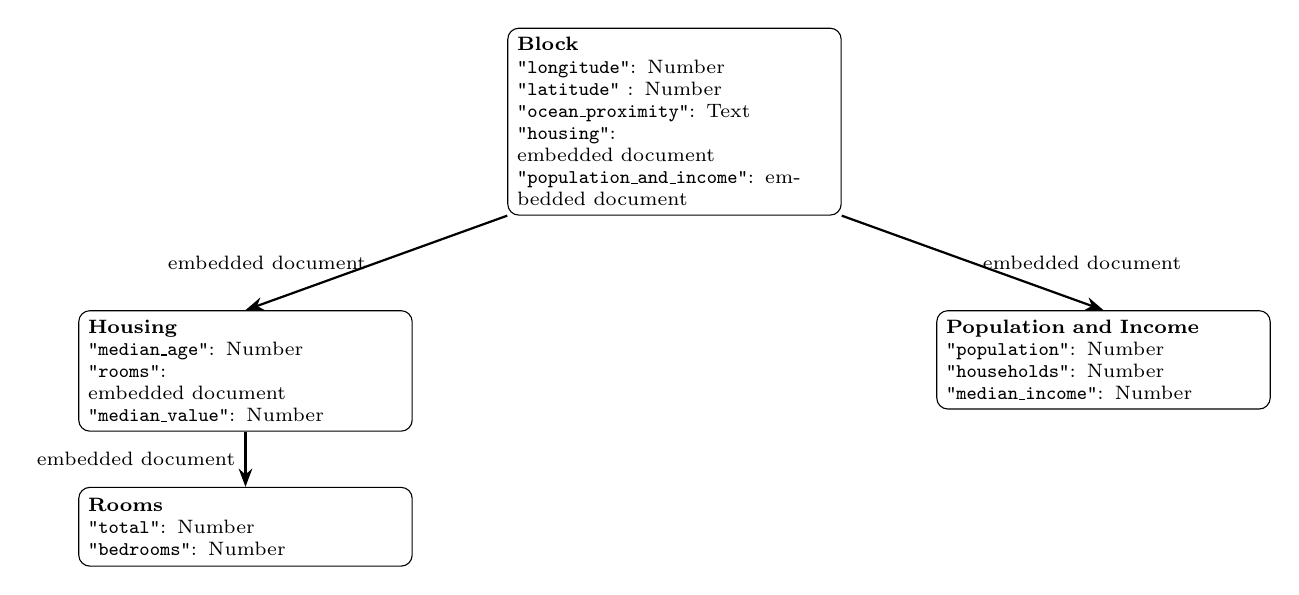
\begin{tikzpicture}[
    scale=0.5, % Scale down the diagram
    every node/.style={transform shape}, % Ensure scaling doesn't distort text
    font=\scriptsize, % Small font for compact layout
    box/.style={draw, rounded corners, text width=4cm, align=left, minimum height=1cm, node distance=0.7cm},
    arrow/.style={->, thick, >=Stealth},
    every node/.style={align=left}
]

% block 
\node[box] (root) {
    \textbf{Block} \\
    \texttt{"longitude"}: Number \\
    \texttt{"latitude"} : Number \\
    \texttt{"ocean\_proximity"}: Text\\
    \texttt{"housing"}:\\ {embedded document} \\
    \texttt{"population\_and\_income"}: {embedded document}
};

% Housing subdocument
\node[box, below left=1.2cm and 1.2cm of root] (housing) {
    \textbf{Housing} \\
    \texttt{"median\_age"}: Number \\
    \texttt{"rooms"}: \\{embedded document} \\
    \texttt{"median\_value"}: Number
};

% Rooms subdocument
\node[box, below=of housing] (rooms) {
    \textbf{Rooms} \\
    \texttt{"total"}: Number \\
    \texttt{"bedrooms"}: Number
};

% Population and Income subdocument
\node[box, below right=1.2cm and 1.2cm of root] (pop_income) {
    \textbf{Population and Income} \\
    \texttt{"population"}: Number \\
    \texttt{"households"}: Number \\
    \texttt{"median\_income"}: Number
};

% Draw arrows
\draw[arrow] (root.south west) -- (housing.north) node[midway, left]  {embedded document};
\draw[arrow] (root.south east) -- (pop_income.north) node[midway, right] {embedded document};
\draw[arrow] (housing.south) -- (rooms.north) node[midway, left] {embedded document};
\end{tikzpicture} 
\end{center}

\subsection{Example of a document}
This is a document that it is created in our db after we shaped the csv file:

\textbf{Block:}\\
\noindent
\texttt{\{} \\
\jsonkey{longitude}: \jsonnumber{-122.05}, \\
\jsonkey{latitude}: \jsonnumber{37.37} \\
\jsonkey{ocean\_proximity}: \jsonstring{NEAR BAY},\\
\jsonkey{housing}: \texttt{\{} \\
\hspace*{1em} \jsonkey{median\_age}: \jsonnumber{27}, \\
\hspace*{1em} \jsonkey{rooms}: \texttt{\{} \\
\hspace*{2em} \jsonkey{total}: \jsonnumber{3885}, \\
\hspace*{2em} \jsonkey{total\_bedrooms}: \jsonnumber{661} \\
\hspace*{1em} \texttt{\}}, \\
\hspace*{1em} \jsonkey{median\_value}: \jsonnumber{344700} \\
\texttt{\}}, \\
\jsonkey{population\_and\_income}: \texttt{\{} \\
\hspace*{1em} \jsonkey{population}: \jsonnumber{1537}, \\
\hspace*{1em} \jsonkey{households}: \jsonnumber{606}, \\
\hspace*{1em} \jsonkey{median\_income}: \jsonnumber{6.6085} \\
\texttt{\}} \\
\texttt{\}}

\section{Data Injection}
The dataset we used was already pretty much cleaned, and complete but we needed to shape it. 
For obtaining a .json file from the .csv file we had we had to write a Python program that was able to transform and shape the data the way we wanted. Here is the python code we used:
\vspace{1cm}
\begin{lstlisting}[language=Python]
import pandas as pd
import json

# Load the CSV file
csv_file = "PathTSavedCSVfile"
df = pd.read_csv(csv_file)

# 1. Check for missing data
print("Missing values per column:\n", df.isnull().sum())

# 2. Handle missing data
# We drop the rows with missing values 
df = df.dropna()


# 3. Convert to JSON-compatible structure (as per your earlier schema)
json_data = []
for _, row in df.iterrows():
    document = {
        "longitude": row["longitude"],
        "latitude": row["latitude"],
        "ocean_proximity": row["ocean_proximity"],        
        "housing": {
            "median_age": row["housing_median_age"],
            "rooms": {
                "total": row["total_rooms"],
                "bedrooms": row["total_bedrooms"]
            },
            "median_value": row["median_house_value"]
        },
        "population_and_income": {
            "population": row["population"],
            "households": row["households"],
            "median_income": row["median_income"]
        }
    }
    json_data.append(document)

# 4. Save cleaned JSON
output_file = "California_Housing.json"
with open(output_file, "w") as f:
    json.dump(json_data, f, indent=4)

print(f"Cleaned JSON file saved to {output_file}")
\end{lstlisting}

We then proceeded to create a db and a collection inside it using compass, a graphical tool studied for Mongo DB, to help us: 
\begin{figure}[H]
    \centering
    
\includegraphics[width=1\linewidth]{LaTeX//Images/Compass.png}
    \caption{Db and collection creation}
    \label{fig:enter-label}
\end{figure}
\section{Queries}
In this section we will see the query we have done and why we thought they were interesting. This section is divided into subsection that represents either a query or a set of query done to answer a question. 

\subsection{Exploring our dataset}
\subsubsection*{Problem regarding the id:}
We grouped these types of queries into a single category because, although they are not very challenging, they provide crucial information about our dataset. The website we obtained the dataset from explicitly mentioned that data cleaning would be necessary. Additionally, as described in section 1.1, the website did not provide detailed information on the dataset, prompting us to execute several queries to better understand its structure.\\
At first, we assigned the \texttt{\_id} in MongoDB to the \texttt{latitude} and \texttt{longitude} coordinates. However, although Compass imported the database without any issues, the logs showed errors. Upon further investigation, we discovered that the problem was likely due to non-unique coordinate values for certain blocks. Subsequently, we altered the database architecture by utilizing the \texttt{\_id} automatically generated by Mongo. Following this adjustment, the errors ceased. To verify our hypothesis regarding the cause, we executed a query to group entries by latitude and longitude. This query showed that some blocks are so closely located that they are detected to have identical latitude and longitude coordinates.

\begin{lstlisting}[language=MongoDB]
db.HousePricing.aggregate([
  {
    $group: {
      _id: { latitude: "$latitude", longitude: "$longitude" },
      count: { $sum: 1 }
    }
  },
  {
    $match: {
      count: { $gt: 1 }
    }
  }, 
  { $sort: {count :- 1} }

]);

\end{lstlisting}

the result is the one we expected:

\noindent
\texttt{\{} \\
\jsonkey{location}: \texttt{\{} \\
\hspace*{1em} \jsonkey{latitude}: \jsonnumber{37.8}, \\
\hspace*{1em} \jsonkey{longitude}: \jsonnumber{-122.41} \\
\texttt{\}}, \\
\jsonkey{count}: \jsonnumber{15} \\
\texttt{\}} \\

\noindent
\texttt{\{} \\
\jsonkey{location}: \texttt{\{} \\
\hspace*{1em} \jsonkey{latitude}: \jsonnumber{37.78}, \\
\hspace*{1em} \jsonkey{longitude}: \jsonnumber{-122.44} \\
\texttt{\}}, \\
\jsonkey{count}: \jsonnumber{11} \\
\texttt{\}}
... 

\subsubsection*{Ocean_proximity values}
A subsequent investigation can be conducted to determine the categories available for ocean proximity in our databases, as the website from which we downloaded the db did not provide this information, which is essential to clarify before commencing the main analysis.

\begin{lstlisting}[language=MongoDB]
db.HousePricing. aggregate([
{$group: {
_id: "$ocean_proximity",
}
}
1);
\end{lstlisting}

\textbf{Result:} \\
\noindent
\texttt{\{} \\
\jsonkey{ocean\_proximity}: \jsonstring{INLAND} \\
\texttt{\}} \\

\noindent
\texttt{\{} \\
\jsonkey{ocean\_proximity}: \jsonstring{NEAR BAY} \\
\texttt{\}} \\

\noindent
\texttt{\{} \\
\jsonkey{ocean\_proximity}: \jsonstring{NEAR OCEAN} \\
\texttt{\}} \\

\noindent
\texttt{\{} \\
\jsonkey{ocean\_proximity}: \jsonstring{ISLAND} \\
\texttt{\}} \\

\noindent
\texttt{\{} \\
\jsonkey{ocean\_proximity}: \jsonstring{<1H OCEAN} \\
\texttt{\}} \\

\subsubsection*{Housing price capped at 501000\$}
The final straightforward query we conducted aimed to verify our suspicion that house prices are limited to 501000\$. To confirm this, we executed the following query:
\begin{lstlisting}[language=MongoDB]
db.HousePricing.countDocuments({
    "housing.median_value": { $gt: 500001 }
});
\end{lstlisting}
and the return was 0 while for the same query with value equal to 500001 the value was 958. This is important because it means that when doing statistic on this we need to remember to remove the richest houses. 

\subsection{Island}
Although we are enthusiasts of California, we were unaware of the existence of any populated islands. This piqued our curiosity, leading us to investigate the number of blocks on the island by executing this query:
\begin{lstlisting}[language=MongoDB]
db.HousePricing.countDocuments({
    "ocean_proximity": "ISLAND"
});
\end{lstlisting}
The outcome is 5. 
We became intrigued to determine whether they all originated from the same island, prompting us to execute this query:
\begin{lstlisting}[language=MongoDB]
db.HousePricing.find({ocean_proximity:"ISLAND"}, {_id : 0, longitude: 1, latitude:1})
\end{lstlisting}
and found that all values of longitude and latitude that are very close to each other: 

\noindent
\texttt{\{} \\
\jsonkey{longitude}: \jsonnumber{-118.32}, \\
\jsonkey{latitude}: \jsonnumber{33.35} \\
\texttt{\}} \\


\noindent
\texttt{\{} \\
\jsonkey{longitude}: \jsonnumber{-118.33}, \\
\jsonkey{latitude}: \jsonnumber{33.34} \\
\texttt{\}} \\


\noindent
\texttt{\{} \\
\jsonkey{longitude}: \jsonnumber{-118.32}, \\
\jsonkey{latitude}: \jsonnumber{33.33} \\
\texttt{\}} \\


\noindent
\texttt{\{} \\
\jsonkey{longitude}: \jsonnumber{-118.32}, \\
\jsonkey{latitude}: \jsonnumber{33.34} \\
\texttt{\}} \\


\noindent
\texttt{\{} \\
\jsonkey{longitude}: \jsonnumber{-118.48}, \\
\jsonkey{latitude}: \jsonnumber{33.43} \\
\texttt{\}}

We concluded that they are all part of the same big inhabited island.
The actual island is called Santa Catalina and it is one of the few inhabited islands of California.
\begin{figure}[H]
    \centering
    
\includegraphics[width=1\linewidth]{LaTeX//Images/Avalon_Santa_Catalina_Island.png}
    \caption{Avalon, Santa Catalina Island}
    \label{fig:enter-label}
\end{figure}

We were interested in comparing the median house value on this island to those throughout the rest of California, so we examined this: 
\begin{lstlisting}[language=MongoDB]
db.HousePricing.aggregate([
    {$match: {ocean_proximity: "ISLAND" }},
  {
    $group: {
      _id: null, 
      median_house_value: { $avg: "$housing.median_value" } 
    }
  }
])
\end{lstlisting}
this returned the value 380440, which is much higher than the general one of California we get by removing the first constraint: 
\begin{lstlisting}[language=MongoDB]
db.HousePricing.aggregate([
  {
    $group: {
      _id: null, 
      median_house_value: { $avg: "$housing.median_value" } 
    }
  }
])
\end{lstlisting}
The result obtained from this query is roughly 206864. This aligns with our expectations, as San Catalina appears to be a truly beautiful island from the photos.



\subsection{Population distribution}
We were curious to see about the distribution of the population there. Therefore, we executed a query to retrieve the 1000 most densely populated blocks, categorizing them by their ocean\_proximity values. This allows us to verify whether the densest areas in California are indeed located near the coast, as we assumed based on our limited knowledge of the state.:

\begin{lstlisting}[language=MongoDB]
db.HousePricing.aggregate([
{$sort : { population : -1}},
{$limit : 1000},
{$group : {_id : "$ocean_proximity" , population : {$sum : "$population_and_income. population"}} }
]);
\end{lstlisting}

with this query we got these results:

\noindent
\texttt{\{} \\
\jsonkey{ocean\_proximity}: \jsonstring{<1H OCEAN}, \\
\jsonkey{population\_and\_income}: \texttt{\{} \\
\hspace*{1em} \jsonkey{population}: \jsonnumber{164759} \\
\texttt{\}} \\
\texttt{\}} \\


\noindent
\texttt{\{} \\
\jsonkey{ocean\_proximity}: \jsonstring{INLAND}, \\
\jsonkey{population\_and\_income}: \texttt{\{} \\
\hspace*{1em} \jsonkey{population}: \jsonnumber{58631} \\
\texttt{\}} \\
\texttt{\}} \\


\noindent
\texttt{\{} \\
\jsonkey{ocean\_proximity}: \jsonstring{NEAR BAY}, \\
\jsonkey{population\_and\_income}: \texttt{\{} \\
\hspace*{1em} \jsonkey{population}: \jsonnumber{998872} \\
\texttt{\}} \\
\texttt{\}}

This is the result we were expecting, knowing there are a lot of big cities in California near the ocean: 

\begin{figure}[H]
    \centering
    
\includegraphics[width=0.5\linewidth]{LaTeX/Images/California_Density_Population.png}
    \caption{{Image taken from: \href{https://www.geocurrents.info/blog/tag/california-population/}{California population distribution}}}
    \label{fig:enter-label}
\end{figure}

\subsection{Most populated areas}
Now we are interested in retrieving the areas/cities that are actually the most populated.To do so, we will group each block by the longitude and latitude with an integer approximation. This is the resulting query:

\begin{lstlisting}[language=MongoDB]
db.HousePricing.aggregate([
    {
        $group: {
            _id: {
                longitude: { $round: ["$longitude", 0] }, 
                latitude: { $round: ["$latitude", 0] }   
            },
            totalPopulation: { $sum: "$population_and_income.population" },
        }
    },
    {
        $sort: { totalPopulation: -1 } 
    },
    {
        $limit: 4 
    }
]);
\end{lstlisting}

with results: 

\noindent
\texttt{\{} \\
\jsonkey{location}: \texttt{\{} \\
\hspace*{1em} \jsonkey{longitude}: \jsonnumber{-118}, \\
\hspace*{1em} \jsonkey{latitude}: \jsonnumber{34} \\
\texttt{\}}, \\
\jsonkey{totalPopulation}: \jsonnumber{10685969} \\
\texttt{\}} \\


\noindent
\texttt{\{} \\
\jsonkey{location}: \texttt{\{} \\
\hspace*{1em} \jsonkey{longitude}: \jsonnumber{-122}, \\
\hspace*{1em} \jsonkey{latitude}: \jsonnumber{38} \\
\texttt{\}}, \\
\jsonkey{totalPopulation}: \jsonnumber{3690156} \\
\texttt{\}} \\


\noindent
\texttt{\{} \\
\jsonkey{location}: \texttt{\{} \\
\hspace*{1em} \jsonkey{longitude}: \jsonnumber{-117}, \\
\hspace*{1em} \jsonkey{latitude}: \jsonnumber{33} \\
\texttt{\}}, \\
\jsonkey{totalPopulation}: \jsonnumber{2433763} \\
\texttt{\}} \\


\noindent
\texttt{\{} \\
\jsonkey{location}: \texttt{\{} \\
\hspace*{1em} \jsonkey{longitude}: \jsonnumber{-122}, \\
\hspace*{1em} \jsonkey{latitude}: \jsonnumber{37} \\
\texttt{\}}, \\
\jsonkey{totalPopulation}: \jsonnumber{2181651} \\
\texttt{\}}


Upon examining the results, we identified the coordinates for the most densely populated cities in California. The first coordinate corresponds to Los Angeles, followed by the second for San Francisco, the third for San Diego, and the fourth for San Jose.

\begin{figure}[H]
    \centering
    
\includegraphics[width=1\linewidth]{LaTeX//Images/LosAngeles.png}
    \caption{Los Angeles, Hollywood}
    \label{fig:enter-label}
\end{figure}



\subsection{Which is older, SF or LA?}
We have always seen San Francisco (SF) and Los Angeles (LA) as modern cities where house are all relatively new so we were curious to see between the 2 which contained the oldest housing according to our db.  
So we run these 2 queries: 

\begin{lstlisting}[language=MongoDB]
db.HousePricing.aggregate([
  {
    $match: {
      longitude: { $gte: -118.5 , $lte: -117.5 },
      latitude: { $gte: 33.5, $lte: 34.5 }
    }
  },
  {
    $group: {
      _id: "Los Angeles",
      averageMedianAge: { $avg: "$housing.median_age" }
    }
  }
]);
\end{lstlisting}

and 
\begin{lstlisting}[language=MongoDB]
db.HousePricing.aggregate([
  {
    $match: {
      longitude: { $gte: -122.5, $lte: -121.4 },
      latitude: { $gte: 37.5, $lte: 38.4 }
    }
  },
  {
    $group: {
      _id: "San Francisco",
      averageMedianAge: { $avg: "$housing.median_age" }
    }
  }
]);
\end{lstlisting}

finding the result that the 2 cities and suburbs are basically infrastructurally modern the same:

\noindent
\texttt{\{} \\
\jsonkey{location}: \jsonstring{Los Angeles}, \\
\jsonkey{averageMedianAge}: \jsonnumber{31.760942291608586} \\
\texttt{\}}
\noindent
\texttt{\{} \\
\jsonkey{location}: \jsonstring{San Francisco}, \\
\jsonkey{averageMedianAge}: \jsonnumber{35.27605834222697} \\
\texttt{\}}


\subsection{Home Price-to-Income Ratio}
Now we were curious to compare the 2 most renown city of California for the median income compared to the median house value. Although the median house value does not represent exactly the cost of living for this kind of database it is the best we can do. So we run these 2 queries:

\begin{lstlisting}[language=MongoDB]
db.HousePricing.aggregate([
  {
    $match: {
      longitude: { $gte: -118.5 , $lte: -117.5 },
      latitude: { $gte: 33.5, $lte: 34.5 }
    }
  },
  {
    $group: {
      _id: "Los Angeles",
       averageIncomeToLivingCostRatio: {
                $avg: {
                    $divide: ["$population_and_income.median_income", "$housing.median_value"]
                }
            }
    }
  }
]);
\end{lstlisting}

and 
\begin{lstlisting}[language=MongoDB]
db.HousePricing.aggregate([
    {
        $match: {
            "longitude": { $gte: -122.5, $lte: -121.5 },
            "latitude": { $gte: 37.5, $lte: 38.5 }
        }
    },
    {
        $group: {
            _id: "San Francisco",
            averageIncomeToLivingCostRatio: {
                $avg: {
                    $divide: ["$population_and_income.median_income", "$housing.median_value"]
                }
            }
        }
    }
]);

\end{lstlisting}

and found these results:
\noindent
\texttt{\{} \\
\jsonkey{location}: \jsonstring{Los Angeles}, \\
\jsonkey{averageIncomeToLivingCostRatio}: \jsonnumber{0.000018154235715803063} \\
\texttt{\}}
\noindent
\texttt{\{} \\
\jsonkey{location}: \jsonstring{San Francisco}, \\
\jsonkey{averageIncomeToLivingCostRatio}: \jsonnumber{0.000018695463849772272} \\
\texttt{\}}

In this case we found a significant difference in this ratio telling us that the most affordable city is actually SF.

\begin{figure}[H]
    \centering
    
\includegraphics[width=1\linewidth]{LaTeX//Images/San_Francisco.png}
    \caption{San Francisco}
    \label{fig:enter-label}
\end{figure}

The fact that San Francisco has an higher Home Price-to-Income Ratio is also confirmed also in this study and it is also true today: \href{https://www.voronoiapp.com/real-estate/Los-Angeles-Has-The-Highest-Home-Price-to-Income-Ratio-In-The-US--2717?utm_source=chatgpt.com}{link}. 

\subsection{Most affordable block near SF}
Since as good computer scientist we always dream about living in the Silicon Valley we were curious also to see what was the most affordable block near San Francisco so we run this query: 
\begin{lstlisting}[language=MongoDB]
db.HousePricing.aggregate([
    {
        $match: {
            "longitude": { $gte: -122.5, $lte: -121.5 },
            "latitude": { $gte: 37.5, $lte: 38.5 }
        }
    },
    {
        $sort: { "housing.median_value": 1 } // Sort by median value in ascending order
    },
    {
        $limit: 1 // Take the first block with the lowest median value
    },
    {
        $project: {
            _id: 1,
            "longitude": 1,
            "latitude": 1,
            "housing.median_value": 1
        }
    }
]);
\end{lstlisting}
And found this result: \\ 
\noindent
\texttt{\{} \\
\jsonkey{\_id}: \jsonstring{ObjectId('674e07b554da08875740ddd2')}, \\
\jsonkey{longitude}: \jsonnumber{-122.32}, \\
\jsonkey{latitude}: \jsonnumber{37.93}, \\
\jsonkey{housing}: \texttt{\{} \\
\hspace*{1em} \jsonkey{median\_value}: \jsonnumber{22500} \\
\texttt{\}} \\

This area is not actually in the center of San Francisco but it  is not even so far. From the center of SF we it is approximately 30 minutes.

\subsection{Average person per household}
 Now we were curious to have some data about the person per household ratio querying the avg of this ratio and the std deviation in the various block to know more or less how numerous are the families there:
\begin{lstlisting}[language=MongoDB]
db.HousePricing.aggregate([
    {
        $project: {
            person_per_household: {
                $cond: [
                    { $ne: ["$population_and_income.households", 0] }, // Avoid division by zero
                    { $divide: ["$population_and_income.population", "$population_and_income.households"] },
                    null // If households is 0, set ratio to null
                ]
            }
        }
    },
    {
        $match: {
            person_per_household: { $ne: null } // Exclude null ratios (e.g., where households = 0)
        }
    },
    {
        $group: {
            _id: null,
            avgRatio: { $avg: "$person_per_household" },
            stdDevRatio: { $stdDevPop: "$person_per_household" }
        }
    }
]);
\end{lstlisting}
this is his result:
\textbf{Block:}\\
\noindent
\texttt{\{} \\
\jsonkey{\_id}: \jsonnull{null}, \\
\jsonkey{avgRatio}: \jsonnumber{3.071532851191042}, \\
\jsonkey{stdDevRatio}: \jsonnumber{10.438013767697397} \\
\texttt{\}}

We were shocked by the enormous standard deviation so we decides to investigate further with the following query aiming to discover more about the outliers:
\begin{lstlisting}[language=MongoDB]
db.HousePricing.aggregate([
    {
        $project: {
            person_per_household: {
                $divide: ["$population_and_income.population", "$population_and_income.households"]
            }
        }
    },
    {
        $match: {
            person_per_household: { $gt: 20 }
        }
    },
]);
\end{lstlisting}

And we discovered that there are outliers data like these ones:
\noindent
\texttt{\{} \\
\jsonkey{\_id}: \jsonstring{ObjectId('674e07b554da08875740e3c6')}, \\
\jsonkey{person\_per\_household}: \jsonnumber{599.7142857142857} \\
\texttt{\}}
... 
\noindent
\texttt{\{} \\
\jsonkey{\_id}: \jsonstring{ObjectId('674e07b654da088757412045')}, \\
\jsonkey{person\_per\_household}: \jsonnumber{1243.3333333333333} \\
\texttt{\}}

So we decided to make a query like the first one but elliminating the outliers:

\begin{lstlisting}[language=MongoDB]
db.HousePricing.aggregate([
    {
        $project: {
            person_per_household: {
                $divide: ["$population_and_income.population", "$population_and_income.households"]
            }
        }
    },
    {
        $match: {
            person_per_household: { $lte: 20 } // Filter out extreme ratios
        }
    },
    {
        $group: {
            _id: null,
            avgPersonPerHousehold: { $avg: "$person_per_household" },
            stdDevPersonPerHousehold: { $stdDevPop: "$person_per_household" }
        }
    }
]);
\end{lstlisting}

\textbf{Block:}\\
\noindent
\texttt{\{} \\
\jsonkey{\_id}: \jsonnull{null}, \\
\jsonkey{avgPersonPerHousehold}: \jsonnumber{2.932484316128325}, \\
\jsonkey{stdDevPersonPerHousehold}: \jsonnumber{0.8698095598200718} \\
\texttt{\}}

This standard deviation actually makes a lot more sense to us now. 

Now we were curious to see why we had this extreme outliers so we run the following easy queries:

\begin{lstlisting}[language=MongoDB]
db.HousePricing.find({ _id: ObjectId('674e07b654da088757412045') }, {longitude:1, latitude:1})
\end{lstlisting}

return: 
\noindent
\texttt{\{} \\
\jsonkey{\_id}: \jsonstring{ObjectId('674e07b554da08875740e3c6')}, \\
\jsonkey{longitude}: \jsonnumber{-120.51}, \\
\jsonkey{latitude}: \jsonnumber{40.41} \\
\texttt{\}}


\begin{lstlisting}[language=MongoDB]
db.HousePricing.find({ _id: ObjectId('674e07b654da088757412045') }, {longitude:1, latitude:1})
\end{lstlisting}



\noindent
\texttt{\{} \\
\jsonkey{\_id}: \jsonstring{ObjectId('674e07b654da088757412045')}, \\
\jsonkey{longitude}: \jsonnumber{-121.98}, \\
\jsonkey{latitude}: \jsonnumber{38.32} \\
\texttt{\}}

Now if we investigate further using a website like \href{Gps coordinates}{https://gps-coordinates.org/} to know what area we are looking at we notice that all of these geographical coordinate correspond to prisons. The first one is High Desert State Prison while the second is California State Prison Solano. So probably they considered the prisoners as a single household.
\begin{figure}[H]
    \centering
    
\includegraphics[width=1\linewidth]{LaTeX//Images/High Desert state prison.png}
    \caption{High desert state prison}
    \label{fig:enter-label}
\end{figure}




\subsection{Home price to income ratio}
We know well that Americans often spend beyond their means. So we thought that an interesting query would be to knows the area in California where people spend the most, relative to their income, on housing. To do so we exploits the trick we used previously to group part of America approximating the latitude and the longitude to one digit:

\begin{lstlisting}[language=MongoDB]
db.HousePricing.aggregate([
    {
        $group: {
            _id: {
                longitude: { $round: ["$longitude", 0] }, 
                latitude: { $round: ["$latitude", 0] }   
            },
            homeprice_to_income: { 
                $avg: { 
                    $divide: ["$housing.median_value", "$population_and_income.median_income"] 
                } 
            }
        }
    },
    {
        $sort: { homeprice_to_income: -1 } 
    }, 
  {
$limit:1
}
]);
\end{lstlisting}

and this is the result:


\noindent
\texttt{\{} \\
\jsonkey{\_id}: \texttt{\{} \\
\hspace*{1em} \jsonkey{longitude}: \jsonnumber{-120}, \\
\hspace*{1em} \jsonkey{latitude}: \jsonnumber{34} \\
\texttt{\}}, \\
\jsonkey{homeprice\_to\_income}: \jsonnumber{88376.19072601027} \\
\texttt{\}}

This points directly to the complex of islands near the bay. At first glance someone could think that are the housing in island. actually if we ran this query:
\begin{lstlisting}[language=MongoDB]
db.HousePricing.aggregate([
    {
        $match: {
            "longitude": { $gte: -120.4, $lte: -119.6 },
            "latitude": { $gte: 33.6, $lte: 34.4 },
            "ocean_proximity": "ISLAND" 
        }
    }
]);
\end{lstlisting}
we don't find any results, and rightfully so since the 2 island are natural reserve. To know so why there is a so  high diproportion there we could run this other query: 

\begin{lstlisting}[language=MongoDB]
db.HousePricing.aggregate([
    {
        $match: {
            "longitude": { $gte: -120.4, $lte: -119.6 },
            "latitude": { $gte: 33.6, $lte: 34.4 }
        }
    },
    {
        $sort: { "population_and_income.median_income": 1 } 
    },
    {
        $project: {
            _id: 0, // Exclude the default _id field
            longitude: 1,
            latitude: 1,
            "housing.median_value": 1,
            "population_and_income.median_income": 1
        }
    }
]);
\end{lstlisting}
this will return 
\textbf{Block:}\\
\noindent
\texttt{\{} \\
\jsonkey{longitude}: \jsonnumber{-119.86}, \\
\jsonkey{latitude}: \jsonnumber{34.38}, \\
\jsonkey{housing}: \texttt{\{} \\
\hspace*{1em} \jsonkey{median\_value}: \jsonnumber{316700} \\
\texttt{\}}, \\
\jsonkey{population\_and\_income}: \texttt{\{} \\
\hspace*{1em} \jsonkey{median\_income}: \jsonnumber{1.5071} \\
\texttt{\}} \\
\texttt{\}} \\

\textbf{Block:}\\
\noindent
\texttt{\{} \\
\jsonkey{longitude}: \jsonnumber{-119.85}, \\
\jsonkey{latitude}: \jsonnumber{34.4}, \\
\jsonkey{housing}: \texttt{\{} \\
\hspace*{1em} \jsonkey{median\_value}: \jsonnumber{37500} \\
\texttt{\}}, \\
\jsonkey{population\_and\_income}: \texttt{\{} \\
\hspace*{1em} \jsonkey{median\_income}: \jsonnumber{2.1652} \\
\texttt{\}} \\
\texttt{\}} \\

\textbf{Block:}\\
\noindent
\texttt{\{} \\
\jsonkey{longitude}: \jsonnumber{-119.69}, \\
\jsonkey{latitude}: \jsonnumber{34.38}, \\
\jsonkey{housing}: \texttt{\{} \\
\hspace*{1em} \jsonkey{median\_value}: \jsonnumber{281300} \\
\texttt{\}}, \\
\jsonkey{population\_and\_income}: \texttt{\{} \\
\hspace*{1em} \jsonkey{median\_income}: \jsonnumber{2.25} \\
\texttt{\}} \\
\texttt{\}}


That are all coordinate of Santa Barbara. The high ratio is due to the fact that Santa Barbara, is one of the most turistic cities of the Bay but does not have big tech company like San Francisco. This lead to a big disproportion to house value and actual income.

\begin{figure}[H]
    \centering
    
\includegraphics[width=1\linewidth]{LaTeX//Images/SantaBarbata.png}
    \caption{Santa Barbara}
    \label{fig:enter-label}
\end{figure}

\subsection{Near block with highest difference in median house value}
Th last query we finded interesting was a query to return the 2 blocks in San Francisco which are near but have the highest differece in median house value. To simplify things we says that to be near the 2 block must have a difference of longitude and latititude which is <= 0.01. So we run this difficult query: 

\begin{lstlisting}[language=MongoDB]
db.HousePricing.aggregate([
    // Step 1: Filter for San Francisco area
    {
        $match: {
            longitude: { $gte: -123, $lte: -122 },
            latitude: { $gte: 37, $lte: 38 }
        }
    },
    // Step 2: Self-join to find nearby blocks
    {
        $lookup: {
            from: "HousePricing",
            as: "neighbors",
            let: { currentId: "$_id", currentLongitude: "$longitude", currentLatitude: "$latitude", currentMedianValue: "$housing.median_value" },
            pipeline: [
                {
                    $match: {
                        $expr: {
                            $and: [
                                { $lte: [{ $abs: { $subtract: ["$longitude", "$$currentLongitude"] } }, 0.01] },
                                { $lte: [{ $abs: { $subtract: ["$latitude", "$$currentLatitude"] } }, 0.01] },
                                { $ne: ["$_id", "$$currentId"] } // Ensure different blocks
                            ]
                        }
                    }
                },
                {
                    $project: {
                        _id: 0,
                        longitude: 1,
                        latitude: 1,
                        neighborMedianValue: "$housing.median_value"
                    }
                }
            ]
        }
    },
    // Step 3: Flatten the results to get pairs of blocks
    {
        $unwind: "$neighbors"
    },
    // Step 4: Compute the absolute difference in median house value
    {
        $addFields: {
            differenceInMedianValue: {
                $abs: { $subtract: ["$housing.median_value", "$neighbors.neighborMedianValue"] }
            }
        }
    },
    // Step 5: Sort by the difference in descending order
    {
        $sort: { differenceInMedianValue: -1 }
    },
    // Step 6: Limit to get just 1 result. 
    {
        $limit: 1
    },
    // Step 7: Project the final output
    {
        $project: {
            _id: 0,
            block1: {
                longitude: "$longitude",
                latitude: "$latitude",
                medianValue: "$housing.median_value"
            },
            block2: {
                longitude: "$neighbors.longitude",
                latitude: "$neighbors.latitude",
                medianValue: "$neighbors.neighborMedianValue"
            },
            differenceInMedianValue: 1
        }
    }
]);
\end{lstlisting}

and we finded this results: \\
\noindent
\texttt{\{} \\
\jsonkey{differenceInMedianValue}: \jsonnumber{467501}, \\
\jsonkey{block1}: \texttt{\{} \\
\hspace*{1em} \jsonkey{longitude}: \jsonnumber{-122.41}, \\
\hspace*{1em} \jsonkey{latitude}: \jsonnumber{37.78}, \\
\hspace*{1em} \jsonkey{medianValue}: \jsonnumber{32500} \\
\texttt{\}}, \\
\jsonkey{block2}: \texttt{\{} \\
\hspace*{1em} \jsonkey{longitude}: \jsonnumber{-122.41}, \\
\hspace*{1em} \jsonkey{latitude}: \jsonnumber{37.79}, \\
\hspace*{1em} \jsonkey{medianValue}: \jsonnumber{500001} \\
\texttt{\}} \\
\texttt{\}}




As we can see on google maps the richest area actually correspond to one of the most renown square of San Francisco, Union square. In Union square there are not actually not so many housing (being that area mostly dedicated to expensive hotel and shops) but the one we have are all over the max limit of 501000\$. The other more periferic area instead is probably corresponding to China Town, that is famous instead for the organized crime especially in the 90s, so maybe the low price is due to that. 

\begin{figure}[H]
    \centering
    
\includegraphics[width=1\linewidth]{LaTeX//Images/UnionSquare.png}
    \caption{Union Square}
    \label{fig:enter-label}
\end{figure}



\chapter{Chapter one}
\label{ch:chapter_one}%
% The \label{...}% enables to remove the small indentation that is generated, always leave the % symbol.

In this chapter additional useful information are reported.

\section{Sections and subsections}
\label{sec:section_name}
Chapters are typically subdivided into sections and subsections, and, optionally,
subsubsections, paragraphs and subparagraphs.
All can have a title, but only sections and subsections are numbered.
A new section is created by the command
\begin{verbatim}
\section{Title of the section}
\end{verbatim}
The numbering can be turned off by using \verb|\section*{}|.
\\
A new subsection is created by the command
\begin{verbatim}
\subsection{Title of the subsection}
\end{verbatim}
and, similarly, the numbering can be turned off by adding an asterisk as follows 
\begin{verbatim}
\subsection*{}
\end{verbatim}

\section{Equations}
\label{sec:eqs}
This section gives some examples of writing mathematical equations in your thesis.

Maxwell's equations read:
\begin{subequations}
    \label{eq:maxwell}
    \begin{align}[left=\empheqlbrace]
    \nabla\cdot \bm{D} & = \rho, \label{eq:maxwell1} \\
    \nabla \times \bm{E} +  \frac{\partial \bm{B}}{\partial t} & = \bm{0}, \label{eq:maxwell2} \\
    \nabla\cdot \bm{B} & = 0, \label{eq:maxwell3} \\
    \nabla \times \bm{H} - \frac{\partial \bm{D}}{\partial t} &= \bm{J}. \label{eq:maxwell4}
    \end{align}
\end{subequations}

Equation~\eqref{eq:maxwell} is automatically labeled by \texttt{cleveref},
as well as Equation~\eqref{eq:maxwell1} and Equation~\eqref{eq:maxwell3}.
Thanks to the \verb|cleveref| package, there is no need to use \verb|\eqref|.
Remember that Equations have to be numbered only if they are referenced in the text.

Equations~\eqref{eq:maxwell_multilabels1}, \eqref{eq:maxwell_multilabels2}, \eqref{eq:maxwell_multilabels3}, and \eqref{eq:maxwell_multilabels4} show again Maxwell's equations without brace:
\begin{align}
    \nabla\cdot \bm{D} & = \rho, \label{eq:maxwell_multilabels1} \\
    \nabla \times \bm{E} +  \frac{\partial \bm{B}}{\partial t} &= \bm{0}, \label{eq:maxwell_multilabels2} \\
    \nabla\cdot \bm{B} & = 0, \label{eq:maxwell_multilabels3} \\
    \nabla \times \bm{H} - \frac{\partial \bm{D}}{\partial t} &= \bm{J} \label{eq:maxwell_multilabels4}.
\end{align}

Equation~\eqref{eq:maxwell_singlelabel} is the same as before,
but with just one label:
\begin{equation}
    \label{eq:maxwell_singlelabel}
    \left\{
    \begin{aligned}
    \nabla\cdot \bm{D} & = \rho, \\
    \nabla \times \bm{E} +  \frac{\partial \bm{B}}{\partial t} &= \bm{0},\\
    \nabla\cdot \bm{B} & = 0, \\
    \nabla \times \bm{H} - \frac{\partial \bm{D}}{\partial t} &= \bm{J}.
    \end{aligned}
    \right.
\end{equation}

\section{Figures, Tables and Algorithms}
Figures, Tables and Algorithms have to contain a Caption that describe their content, and have to be properly reffered in the text.

\subsection{Figures}
\label{subsec:figures}

For including pictures in your text you can use \texttt{TikZ} for high-quality hand-made figures,
or just include them as usual with the command
\begin{verbatim}
\includegraphics[options]{filename.xxx}
\end{verbatim}
Here xxx is the correct format, e.g. \verb|.png|, \verb|.jpg|, \verb|.eps|, \dots.

\begin{figure}[H]
    \centering
    
\includegraphics[width=0.3\textwidth]{logo_polimi_scritta.eps}
    \caption{Caption of the Figure to appear in the List of Figures.}
    \label{fig:quadtree}
\end{figure}

Thanks to the \texttt{\textbackslash subfloat} command, a single figure, such as Figure~\ref{fig:quadtree},
can contain multiple sub-figures with their own caption and label, e.g. \color{black} Figure~\ref{fig:polimi_logo1} and Figure~\ref{fig:polimi_logo2}. 

\begin{figure}[H]
    \centering
    \subfloat[One PoliMi logo.\label{fig:polimi_logo1}]{
        
\includegraphics[scale=0.5]{Images/logo_polimi_scritta.eps}
    }
    \quad
    \subfloat[Another one PoliMi logo.\label{fig:polimi_logo2}]{
        
\includegraphics[scale=0.5]{Images/logo_polimi_scritta2.eps}
    }
    \caption[Shorter caption]{This is a very long caption you don't want to appear in the List of Figures.}
    \label{fig:quadtree2}
\end{figure}


\subsection{Tables}
\label{subsec:tables}

Within the environments \texttt{table} and  \texttt{tabular} you can create very fancy tables as the one shown in Table~\ref{table:example}.
\begin{table}[H]
    \caption*{\textbf{Title of Table (optional)}}
    \centering 
    \begin{tabular}{|p{3em} c c c |}
    \hline
    \rowcolor{bluepoli!40} % comment this line to remove the color
     & \textbf{column 1} & \textbf{column 2} & \textbf{column 3} \T\B \\
    \hline \hline
    \textbf{row 1} & 1 & 2 & 3 \T\B \\
    \textbf{row 2} & $\alpha$ & $\beta$ & $\gamma$ \T\B\\
    \textbf{row 3} & alpha & beta & gamma \B\\
    \hline
    \end{tabular}
    \\[10pt]
    \caption{Caption of the Table to appear in the List of Tables.}
    \label{table:example}
\end{table}

You can also consider to highlight selected columns or rows in order to make tables more readable.
Moreover, with the use of \texttt{table*} and the option \texttt{bp} it is possible to align them at the bottom of the page. One example is presented in Table~\ref{table:exampleC}. 

\begin{table}[H]
\centering 
    \begin{tabular}{|p{3em} | c | c | c | c | c | c|}
    \hline
%    \rowcolor{bluepoli!40}
     & \textbf{column1} & \textbf{column2} & \textbf{column3} & \textbf{column4} & \textbf{column5} & \textbf{column6} \T\B \\
    \hline \hline
    \textbf{row1} & 1 & 2 & 3 & 4 & 5 & 6 \T\B\\
    \textbf{row2} & a & b & c & d & e & f \T\B\\
    \textbf{row3} & $\alpha$ & $\beta$ & $\gamma$ & $\delta$ & $\phi$ & $\omega$ \T\B\\
    \textbf{row4} & alpha & beta & gamma & delta & phi & omega \B\\
    \hline
    \end{tabular}
    \\[10pt]
    \caption{Highlighting the columns}
    \label{table:exampleC}
\end{table}

\begin{table}[H]
\centering 
    \begin{tabular}{|p{3em} c c c c c c|}
    \hline
%    \rowcolor{bluepoli!40}
     & \textbf{column1} & \textbf{column2} & \textbf{column3} & \textbf{column4} & \textbf{column5} & \textbf{column6} \T\B \\
    \hline \hline
    \textbf{row1} & 1 & 2 & 3 & 4 & 5 & 6 \T\B\\
    \hline
    \textbf{row2} & a & b & c & d & e & f \T\B\\
    \hline
    \textbf{row3} & $\alpha$ & $\beta$ & $\gamma$ & $\delta$ & $\phi$ & $\omega$ \T\B\\
    \hline
    \textbf{row4} & alpha & beta & gamma & delta & phi & omega \B\\
    \hline
    \end{tabular}
    \\[10pt]
    \caption{Highlighting the rows}
    \label{table:exampleR}
\end{table}

\subsection{Algorithms}
\label{subsec:algorithms}

Pseudo-algorithms can be written in \LaTeX{} with the \texttt{algorithm} and \texttt{algorithmic} packages.
An example is shown in Algorithm~\ref{alg:var}.
\begin{algorithm}[H]
    \label{alg:example}
    \caption{Name of the Algorithm}
    \label{alg:var}
    \label{protocol1}
    \begin{algorithmic}[1]
    \STATE Initial instructions
    \FOR{$for-condition$}
    \STATE{Some instructions}
    \IF{$if-condition$}
    \STATE{Some other instructions}
    \ENDIF
    \ENDFOR
    \WHILE{$while-condition$}
    \STATE{Some further instructions}
    \ENDWHILE
    \STATE Final instructions
    \end{algorithmic}
\end{algorithm} 

\vspace{5mm}

\section{Theorems, propositions and lists}

\subsection{Theorems}
Theorems have to be formatted as:
\begin{theorem}
\label{a_theorem}
Write here your theorem. 
\end{theorem}
\textit{Proof.} If useful you can report here the proof.

\subsection{Propositions}
Propositions have to be formatted as:
\begin{proposition}
Write here your proposition.
\end{proposition}

\subsection{Lists}
How to  insert itemized lists:
\begin{itemize}
    \item first item;
    \item second item.
\end{itemize}
How to insert numbered lists:
\begin{enumerate}
    \item first item;
    \item second item.
\end{enumerate}

%-------------------------------------------------------------------------
%	APPENDICES
%-------------------------------------------------------------------------

\cleardoublepage
\addtocontents{toc}{\vspace{2em}} % Add a gap in the Contents, for aesthetics
\appendix
\chapter{Appendix A}
If you need to include an appendix to support the research in your thesis, you can place it at the end of the manuscript.
An appendix contains supplementary material (figures, tables, data, codes, mathematical proofs, surveys, \dots)
which supplement the main results contained in the previous chapters.


% LIST OF FIGURES
\listoffigures

% LIST OF TABLES
\listoftables

\cleardoublepage

\end{document}
